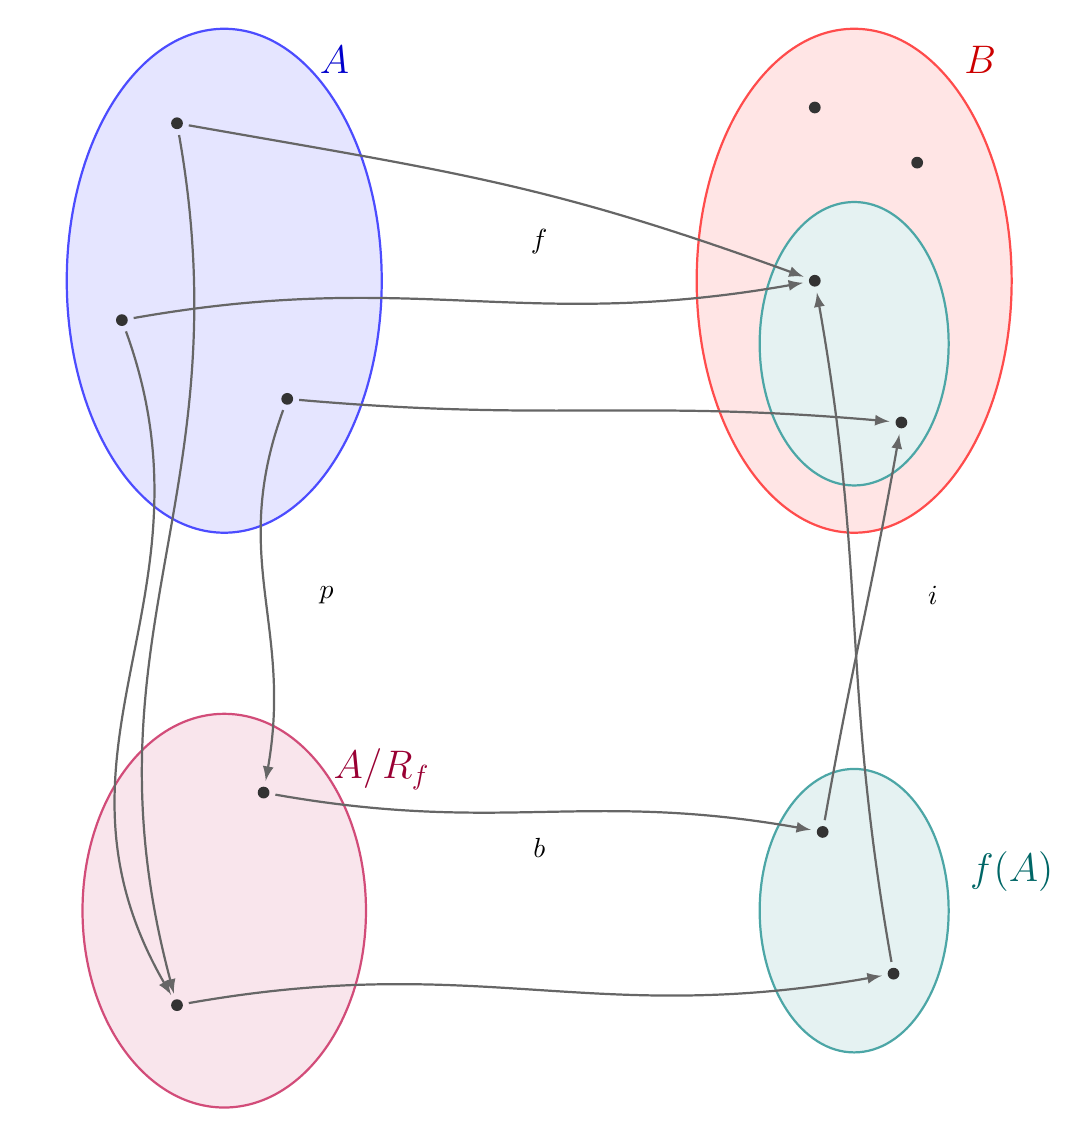
\begin{tikzpicture}[>=latex]

% --- Global TikZ Styles for Consistency ---
\tikzset{
    setA/.style={fill=blue!10, draw=blue!70, thick},
    setB/.style={fill=red!10, draw=red!70, thick},
    setC/.style={fill=purple!10, draw=purple!70, thick}, % Stijl voor A/R_f
    setD/.style={fill=teal!10, draw=teal!70, thick},     % Nieuwe stijl voor f(A)
    labelA/.style={text=blue!80!black, font=\Large\bfseries},
    labelB/.style={text=red!80!black, font=\Large\bfseries},
    labelC/.style={text=purple!80!black, font=\Large\bfseries},
    labelD/.style={text=teal!80!black, font=\Large\bfseries},
    point/.style={circle, fill=black!80, inner sep=1.5pt},
    arrow/.style={
        ->,
        >=latex,
        thick,
        draw=black!60, 
        shorten >=2pt,
        shorten <=2pt
    }
}

% --- Verzameling A (Boven Links) ---
\path[setA] (0, 4) ellipse (2.0cm and 3.2cm);
\node[labelA] at (1.4, 6.8) {$A$};

% Punten in A
\node[point] (p1) at (-0.6, 6.0) {};  % Boven
\node[point] (p2) at (-1.3, 3.5) {};  % Midden-links
\node[point] (p3) at (0.8, 2.5) {};   % Onder-rechts

% --- Verzameling B (Boven Rechts) ---
\path[setB] (8, 4) ellipse (2.0cm and 3.2cm);
\node[labelB] at (9.6, 6.8) {$B$};

% Inner f(A) subset in B (Teal gekleurd om te matchen met de set eronder)
\path[setD] (8, 3.2) ellipse (1.2cm and 1.8cm);

% Punten in B (Outer)
\node[point] (b3) at (7.5, 6.2) {};
\node[point] (b4) at (8.8, 5.5) {};

% Punten in B (Inner / f(A))
\node[point] (b1) at (7.5, 4.0) {};   % Bovenste in subset
\node[point] (b2) at (8.6, 2.2) {};   % Onderste in subset

% --- Verzameling A/R_f (Onder Links) ---
\path[setC] (0, -4) ellipse (1.8cm and 2.5cm);
\node[labelC] at (2.0, -2.2) {$A/R_f$};

% Punten in A/R_f
\node[point] (q1) at (0.5, -2.5) {};  % Bovenste punt
\node[point] (q2) at (-0.6, -5.2) {}; % Onderste punt

% --- Verzameling f(A) (Onder Rechts) ---
\path[setD] (8, -4) ellipse (1.2cm and 1.8cm);
\node[labelD] at (10.0, -3.5) {$f(A)$};

% Punten in f(A)
\node[point] (r1) at (7.6, -3.0) {};  % Bovenste punt
\node[point] (r2) at (8.5, -4.8) {};  % Onderste punt


% ==========================================
% --- Pijlen en Mapping ---
% ==========================================

% f: A -> B (Horizontaal boven)
\draw[arrow] (p1) to[out=-10, in=160, looseness=1.1] (b1);
\draw[arrow] (p2) to[out=10,  in=190, looseness=1.1] (b1);
\draw[arrow] (p3) to[out=-5,  in=175, looseness=1.1] (b2);
\node at (4, 4.5) {$f$};

% p: A -> A/R_f (Verticaal links, pijlen kruisen elkaar)
\draw[arrow] (p1) to[out=-80,  in=105,  looseness=1.1] (q2);
\draw[arrow] (p2) to[out=-70,  in=120, looseness=1.1] (q2);
\draw[arrow] (p3) to[out=-110, in=80,  looseness=1.1] (q1);
\node at (1.3, 0) {$p$};

% b: A/R_f -> f(A) (Horizontaal onder)
\draw[arrow] (q1) to[out=-10, in=170, looseness=1.1] (r1);
\draw[arrow] (q2) to[out=10,  in=190, looseness=1.1] (r2);
\node at (4, -3.2) {$b$};

% i: f(A) -> B (Verticaal rechts, pijlen kruisen elkaar elegant)
\draw[arrow] (r1) to[out=80,  in=-100, looseness=1.1] (b2);
\draw[arrow] (r2) to[out=100, in=-80,  looseness=1.1] (b1);
\node at (9.0, 0) {$i$};

\end{tikzpicture}